	\chapter{Множества.}
\section{Примеры множеств.}
$\bullet$ \textit{\textbf{Множество} --- совокупность объектов, объединённых в одну группу по некоторому признаку.}\\\\
Это не определение, а описание. Понятие множества является первичным и не определяется.\\\\
Основное понятие множеств --- \textbf{отношение принадлежности}. Объекты, составляющие множество, называют \textbf{элементами} этого множества.\\
\begin{example}\\
	\textit{$\N$ --- множество натуральных чисел.\\
		$\Q$ --- множество рациональных чисел.\\
		$\Rm$ --- множество действительных чисел.\\
		$\Z$ --- множество целых чисел.\\
		$\Cm$ --- множество комплексных чисел.}
\end{example}\\\\
Обычно для обозначения множества используют большие буквы латинского алфавита:
\begin{center}
	$A$, $B$, $C$, $U$, $V$, \dots
\end{center}
либо символ $\{\dots\}$.\\\\
Скажем, запись $A=\{x\}$ означает: множество $A$ состоит из элементов $x$. Иногда употребляют развёрнутую запись:
\begin{center}
	$A=\{x\:|\: x$ удовлетворяет условию $P\}$
\end{center}
\begin{example}
	$A=\{x\:|\: x^2-4=0\} \Leftrightarrow A=\{2, -2\}$.
\end{example}\\\\
$\varnothing$ --- пустое множество.\\
$x \in A$ --- $x$ является элементом множества.\\
$y \notin A$ --- $y$ не является элементом множества.\\\\
$\bullet$ \textit{Множество $B$ называют \textbf{подмножеством} множества $A$, если все элементы $B$ являются элементами множества $A$. Записывают $B \subset A$.} \\\\
Очевидно: Если каждый элемент $B$ является элементом $A$ и наоборот, то $A=B$.\\
Коротко $(A \subset B) \wedge (B \subset A) \Rightarrow A=B$.\\\\
$A$ и $\varnothing$ --- \textbf{несобственные} подмножества $A$.\\
Все остальные подмножества называют \textbf{собственными}.\\
\begin{exercise}
	\textit{Конечное множество $\{x\}$ содержит $n$ элементов. Сколько всего подмножеств у этого множества?}
\end{exercise}\\\\
Пусть $A$ и $B$ подмножества множества $M$.
\begin{itemize}
	\item \textit{\textbf{Объединением} $A$ и $B$ называется множество, состоящее из тех и только тех элементов множества $M$, которые содержатся хотя бы в одном из множеств $A$, $B$.}
	\begin{center}
		$A \cup B ::= \{ x \in M \: | \: x \in A \vee x \in B\}$
	\end{center}
	$$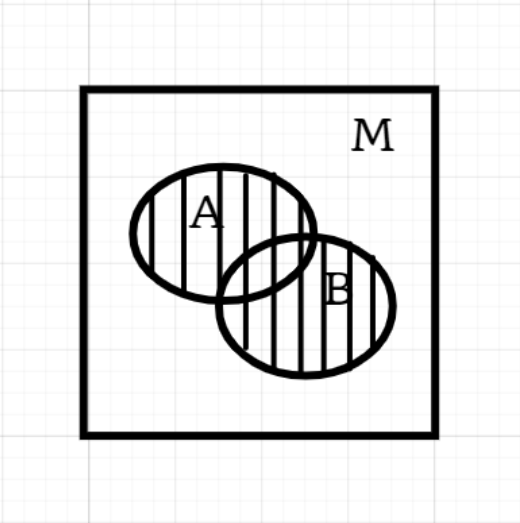
\includegraphics[scale=0.5]{images/img1.png}$$
	\item \textit{\textbf{Пересечением} множеств $A$ и $B$ называется множество, образованное теми и только теми элементами из $M$, которые принадлежат и множеству $A$ и множеству $B$.}
	\begin{center}
		$A \cap B ::= \{ x \in M \: | \: x \in A \wedge x \in B\}$.
	\end{center}
	$$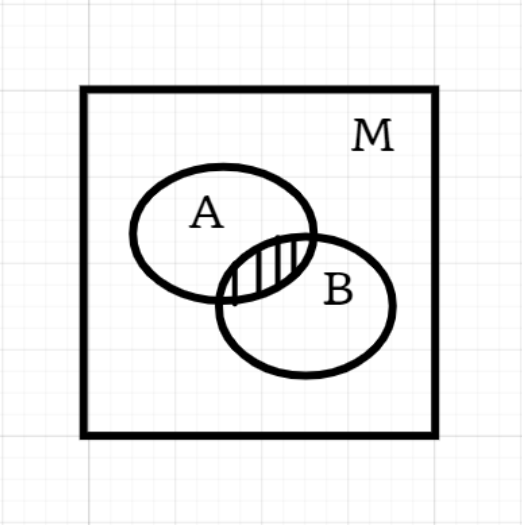
\includegraphics[scale=0.5]{images/img2.png}$$
	\item \textit{\textbf{Разностью} между множеством $A$ и множеством $B$ называют множество, состоящее из тех элементов множества $A$, которые не содержатся в $B$.}
	\begin{center}
		$A \setminus B ::= \{ x \in M \: | \: x \in A \wedge x \notin B\}$
	\end{center}
	$$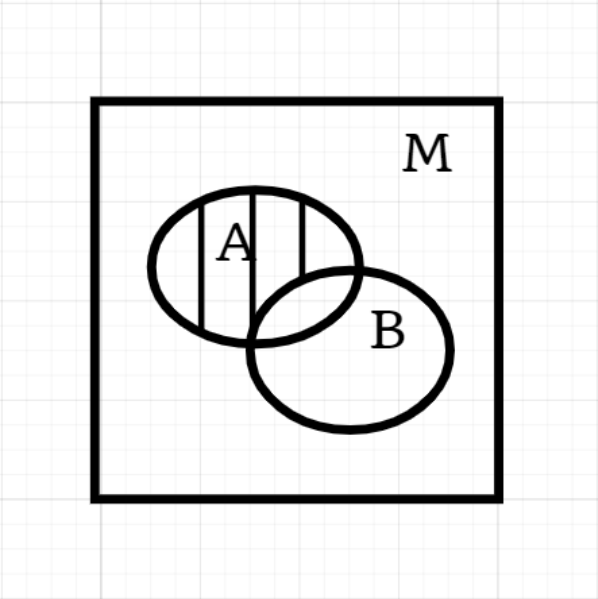
\includegraphics[scale=0.5]{images/img3.png}$$
	\item\textit{\textbf{Дополнением} множества $A$ в множестве $M$ называют разность между $M$ и $A$.}
	\begin{center}
		$C_MA=CA=M\setminus A$
	\end{center}
	$$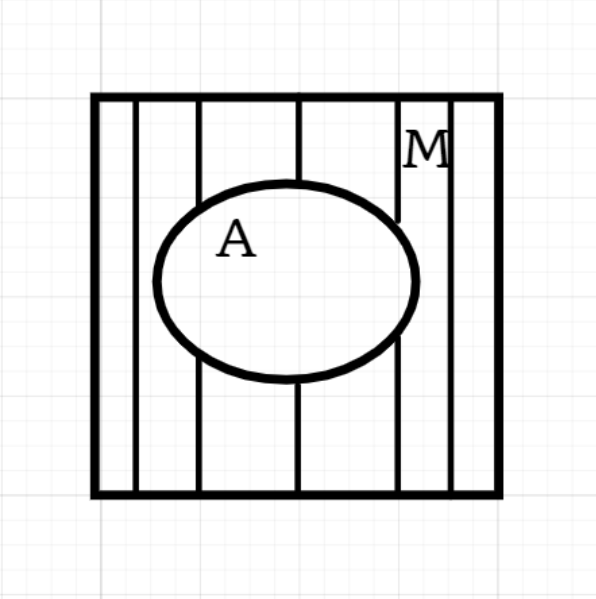
\includegraphics[scale=0.5]{images/img4.png}$$
\end{itemize}
\section{Отображения множеств.}
Пусть заданы два произвольных множества $X$ и $Y$.\\\\
$\bullet$ \textit{\textbf{Отображением} $X$ в $Y$ называется соответствие (правило, закон), которые каждому элементу $x \in X$ сопоставляет некоторый (единственный) элемент $y \in Y$.} \\\\
Обычно заданное отображение обозначают одной буквой, например, $f$, и пишут:
\begin{center}
	$f : X \rightarrow Y;\quad X \xrightarrow{f} Y;\quad f: x \mapsto y; \quad x \xmapsto{f} y.$
\end{center}
$\bullet$ \textit{Элемент $y \in Y$ называетя \textbf{образом} элемента $x \in X$ и обозначается $f(x)$, т. е. $y=f(x)$, а элемент $x$ называется \textbf{прообразом} элемента $y=f(x)$.} \\\\
В связи с этим, для обозначения отображения употребляется символика $x \mapsto f(x), \: y=f(x)$.\\\\
$\bullet$ \textit{Множество $X$, на котором задано отображение $f$, называют \textbf{множеством задания} или \textbf{областью определения} $f$ и иногда для него употребляют символ $D(f)$.} \\\\
$\bullet$ \textit{Множество всех образов отображения $f : X \rightarrow Y$ называют \textbf{множеством значений} отображения $f$ и обозначают $f(X)$ или $E(f)$.} \\\\
$f(X)$ может и не совпадать с $Y$, а быть его подмножеством. Итак $$f(X)=\{ y\:|\:y=f(x), x\in X\}.$$
В зависимости от природы множеств $X$ и $Y$ термин $"$отображение$"$ имеет ряд синонимов: \textit{функция, преобразование, морфизм, оператор, функционал}.\\\\
Таком образом, задание отображения предполагает указание тройки $(X, f, Y)$, где\\
\textit{$X$ --- отображаемое множество или множество задания,\\
	$Y$ --- множество, в которое идёт отображение,\\
	$f$ --- закон, по которому $x \in X \rightarrow y \in Y$.}
\begin{itemize}
	\item \textit{Отображение $f:X \rightarrow Y$ называется \textbf{инъективным отображением} (\textbf{инъекцией, вложением}), если различные элементы множества $X$ имеют и различные образы, т. е. если}
	\begin{center}
		$\forall x_1, x_2 \in X$ и $x_1 \neq x_2 \Rightarrow f(x_1) \neq f(x_2)$.
	\end{center}
	\item \textit{Отображение $f: X \rightarrow Y$ называют \textbf{сюръективным отображением} или \textbf{сюръекцией} (отображение $X$ на $Y$), если $f(X)=Y$, или, другими словами, если каждый элемент из $Y$, является образом при отображении $f$ по крайней мере одного элемента из $X$.
	}
	\item \textit{
		Отображение $f: X \rightarrow Y$ называется \textbf{биективным отображением} или \textbf{биекцией}, если каждый элемент $y \in Y$ является образом при отображении $f$ некоторого, притом единственного элемента из $X$.
	}
\end{itemize}
Анализируя указанные определения и определение отображения, замечаем, что\\\\
$\bullet$ \textit{Отображение $f$ \textbf{биективно} тогда и только тогда, когда оно одновременно \textbf{инъективно и сюръективно}.}\\\\
Другими словами, биекция --- это взаимнооднозначное соответствие между множествами.\\\\
Если $f$ --- биекция и $y \in Y$, то всегда можно указать единственный элемент $x \in X$ такой, что $f(x)=y$. Тем самым определяется некоторое соответствие, отображение $g:Y \rightarrow X$. В силу сюръективности $f$ такой элемент $x$ всегда найдётся, а в силу инъективности он единственный.\\\\
$\bullet$ \textit{Отображение $g$ называют \textbf{обратным отображением} по отношению к $f$ и обозначают символом $f^{-1} : Y \rightarrow X$. (Не путать с $\frac{1}{f}$).}\\\\
Нетрудно увидеть, что $f^{-1}$ --- биекция, если биекцией была $f$.\\\\
$\bullet$ \textit{Отображение $f$, для которого существует отбратное отображение $f^{-1}$, называют \textbf{обратимым}.}\\\\
Из способа построения обратного отображения нетрудно видеть выполнение следующих тождеств:
\begin{center}
	$f^{-1}(f(x))=x, \quad \forall x \in X$\\
	$f(f^{-1}(y))=y, \quad \forall y \in Y$
\end{center}
Пусть теперь заданы два отображения
\begin{center}
	$f : X \rightarrow Y$ и $g : Y \rightarrow Z$,
\end{center}
причём отображение $g$ определено на множестве значений отображения $f$, то можно построить новое отображение $h : X \rightarrow Z$ по следующему правилу
\begin{center}
	$h(x)=g(f(x))$,
\end{center}
т. е. $\forall x \in X$ строим $y=f(x) \in Y$  по этому элементу $y$ находим соответсвующий ему элемент $z=g(y) \in Z$.
$$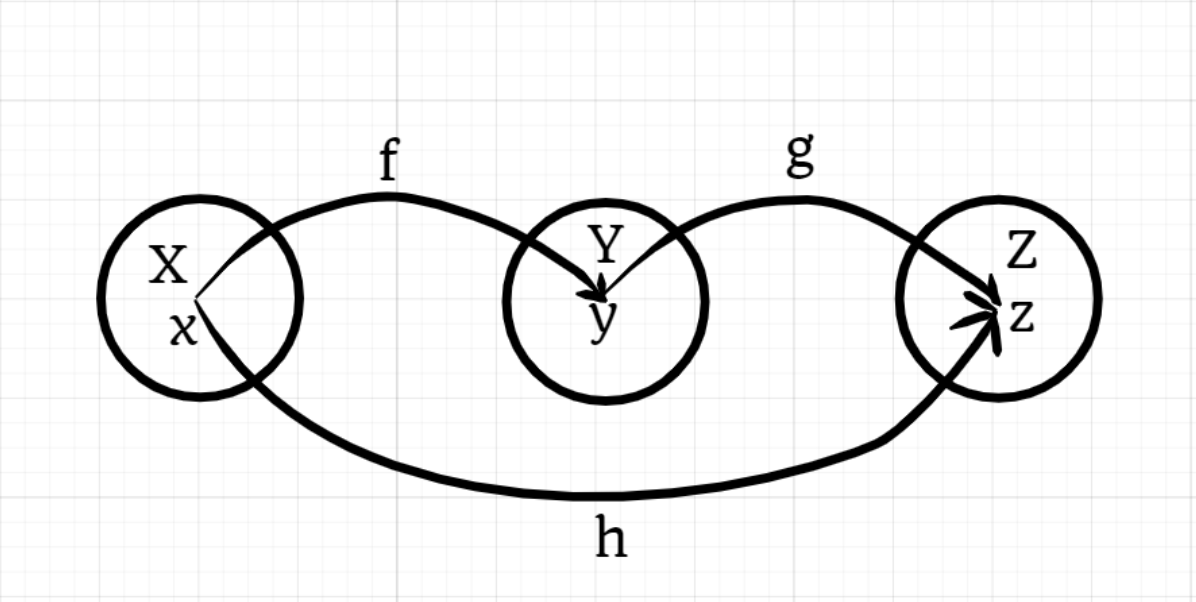
\includegraphics[scale=0.5]{images/img5.png}$$
$\bullet$ \textit{Построенное отображение $h: X \rightarrow Z$ называют \textbf{композицией отображений} $f$ и $g$ и обозначают символом $g \circ f$, то есть}
\begin{center}
	$h = g \circ f.$
\end{center}
Отметим, что важен порядок: $g \circ f \neq f \circ g$.\\
Итак 
\begin{center}
	$h(x)=(g \circ f)(x)=g(f(x))$.
\end{center}
Однако композиция \textbf{ассоциативна}
\begin{center}
	$h \circ ( f \circ g) = (h \circ f) \circ g = h \circ f \circ g$.
\end{center}
Как мы уже отмечали термины $"$отображение$"$ и $"$функция$"$ равносильны. Однако, чаще всего \textit{функцией} называют отображение $f : X \rightarrow Y$, у которого множество $Y$ --- числовое. Для функций используется та же терминология, что и для отображений, имеется в виду то, о чём говорилось выше.\\\\
$\bullet$ \textit{Если $X$ --- числовое множество, то функцию $f$ называют \textit{\textbf{числовой функцией}}. $f^{-1}$ --- \textit{\textbf{обратная функция}}, $g \circ f$ --- \textbf{\textit{композиция функций (сложная функция, суперпозиция)}}}.\\\\
В дальнейшем слово $"$числовая$"$ опускаем, т. к. в ближайшее время изучаем лишь числовые фукции.\\\\
Вообще говоря, следует различать функцию $f$ и элемент $f(x)$, соответствующий элементу $x$ при отображении $f$. Однако по чисто практическим сображениям и в силу традиций это различие часто не принимается во внимание.\\
Так, например, неправильно, но удобно говорить \textit{$"$функция $\sin{x}$$"$}, хотя следует сказать \textit{$"$функция $\sin$$"$}, или \textit{$"$функция $y=x^2$$"$}, хотя нужно \textit{$"$функция, задаваемая формулой $y=x^2$$"$}, или \textit{$"$$f : x \longmapsto x^2$$"$}.\\
Далее мы тоже не будем соблюдать правила и будем  употредлять фразы типа \textit{$"$пусть задана функция $f$$"$} и \textit{$"$пусть задана функция $f(x)$$"$.}\\\\
Функциональную зависимость часто удобно иллюстрировать и изучать геометрически, строя график функции $\Gamma_f$, то есть множество на плоскости
\begin{center}
	$\Gamma_f = \{(x,y) \:|\: x \in D(f), y=f(x)\}$.
\end{center}
к функциям мы впоследствии будем часто возвращаться.
\section{Кванторы.}
Изучение математически становится более простым и удобным, результаты хорошо формулируются и наглядны, если в математических определениях, теоремах и доказательствах часто встречающиеся выражения заменять символами,значками.\\
Так, например, у нас сплошь и рядом будет встречаться выражение \textit{$"$для каждого$"$:(для всех, для любого)}. Вместо этих слов употребляют значок $\forall$, или, как его называют, \textbf{\textit{квантор всеобщности}}.
\begin{enumerate}
	\item[] \textit{\textbf{$\forall x \in X$} \quad --- для любых значений $x$ из множества $X$.}
\end{enumerate}
Квантор существования $\exists$.
\begin{enumerate}
	\item[] \textit{\textbf{$\exists y \notin Y$} \quad --- существует $y$, который не принадлежит множеству $Y$.}
\end{enumerate}
Кроме кванторов, для сокращения записи и в целях обозримости рассуждений, мы часто будем пользоваться символами
\begin{enumerate}
	\item[] \textit{\textbf{$\exists!$} \quad --- существует и единственно, }
	\item[] \textit{\textbf{$::=$} \quad --- равно по определению, }
	\item[] \textit{\textbf{$=::$} \quad --- обозначим через, }
	\item[] \textit{\textbf{$\Rightarrow, \Leftarrow$} \quad --- знак логического следования,}
	\item[] \textit{\textbf{$\Leftrightarrow$} \quad --- знак равносильности, }
	\item[] \textit{\textbf{$\vee$} \quad --- или, }
	\item[] \textit{\textbf{$\wedge$} \quad --- и, }
	\item[] \textit{\textbf{$\rceil$} \quad --- знак отрицания. }
\end{enumerate}
Кроме этих символов будут и другие, которые будут вводиться по мере необходимости.\\\\
Если есть некоторое высказывание, то обратное ему высказывание обозначаем $\rceil P$ (отрицание $P$).\\\\
Нам очень важно будет научиться строить отрицания различных высказываний, содержащих кванторы. При этом полезно знать основные правила.\\
Отрицание к высказыванию \textit{$"$для некоторого $x$ истинно $P(x)$$"$} означает, что \textit{$"$для любого $x$ истинно не $P(x)$$"$}, а отрицание к высказыванию \textit{$"$для любого $x$ истинно $P(x)$$"$} означает, что \textit{$"$найдётся $x$, что не $P(x)$$"$.}\\
Таким образом, символически записываем
\begin{center}
	$\rceil(\exists x P(x)) \Leftrightarrow \forall (\rceil P(x))$\\
	$\rceil(\forall x P(x)) \Leftrightarrow \exists (\rceil P(x))$
\end{center}
т. е. кванторы существования меняются на кванторы всеобщности и наоборот, условие заменяется противоположным.
\section{Счётные и несчётные множества.}
$\bullet$ \textit{Множества $A$ и $B$ называются \textbf{эквивалентными}, если существует биекция $A$ на $B$. Другими словами, множества $A$ и $B$ \textbf{эквивалентны}, если между элементами этих множеств можно остановить взаимно-однозначное соответствие. Запись: $A \sim B$.}\\\\
\textbf{\textit{Свойства:}}
\begin{enumerate}
	\item \textit{симметрия $A \sim B \Rightarrow B \sim A$,}
	\item \textit{рефлексивность $ A \sim A$,}
	\item \textit{транзитивность $A \sim B \wedge B \sim C \Rightarrow A \sim C$.}
\end{enumerate}
\begin{example} $\N \sim \Z$.\\
	$1 \longleftrightarrow 0, \quad 2 \longleftrightarrow 1, \quad 3 \longleftrightarrow -1,\quad \dots,\quad 2m \longleftrightarrow m, \quad 2m+1 \longleftrightarrow -m$.
\end{example}\\\\
Введём обозначение $\I_n ::= \{1, 2, \dots, n\}.$\\\\
$\bullet$ \textit{Множество $A$ называется \textbf{конечным}, если существует $n$ такое, что $A \sim \I_n$ и \textbf{бесконечным} в противном случае.}\\\\
$\bullet$ \textit{Множество $A$ называется \textbf{счётным}, если $A \sim \N$ и \textbf{несчётным}, если $A$ бесконечно, но не счётно.}\\\\
Говорят, что $A$ не более чем счётно, если оно конечно или счётно.\\\\
$\bullet$ \textit{Фукнцию $f : \N \rightarrow \Rm$ называют \textbf{последовательностью} $f : n \longmapsto f(n) =:: a_n \in \Rm$. \quad \quad $(a_n)$}\\\\
Элементы всякого счётного множества можно занумеровать, т. е. представить в виде последовательности. Верно и обратное.
\begin{theorem} Всякое бесконечное подмножество счётного множества само является счётным.
\end{theorem}
\begin{Proof} Пусть $A$ --- счётное множество и $B \subset A$. Т. к. $A$ --- счётно, то $A \sim \N \Rightarrow A=\{a_n\}$. $a_1 \notin B, a_2 \notin B, \dots, a_{n_1} \in B \Rightarrow B=\{a_{n_k}\} \Rightarrow B \sim \N$.
\end{Proof}\\\\
$\bullet$ \textit{\textbf{Объединением или суммой множеств} $A_\alpha, \alpha \in \I_n$ называется множество $S$, что $x \in S$, если $x \in A_\alpha$ хотя бы при одном $\alpha$.}\\\\
Таким образом, любой элемент $x \in A_\alpha$ являющийся и элементом $S$ и множество $S^\prime$ содержит только элементы множества $A_\alpha$.\\
Запись: $S =  \overset{n}{\underset{\alpha=1}{\bigcup}} A_\alpha$\\
Аналогично: $S =  \overset{\infty}{\underset{\alpha=1}{\bigcup}} A_\alpha$\\\\
$\bullet$ \textit{\textbf{Пересечением множеств} $A_\alpha,\ \alpha \in \I_n$, называется множество $P$, что $x \in P$, если $x \in A_\alpha$  $\forall\alpha\in \I_n$.}\\
Элементы Р суть элементы всех множеств $A_\alpha$: $P= \overset{n}{\underset{\alpha=1}{\cap}} A_\alpha$\\
Аналогично: $P =  \overset{\infty}{\underset{\alpha=1}{\bigcap}} A_\alpha$\\
\begin{theorem} 
	Объединеие счётного числа счётных множеств счётно.
\end{theorem}
\begin{Proof}
	$A_1 = x_1^{(1)} \underset{\swarrow}{\rightarrow} x_2^{(1)} \qquad x_3^{(1)} \underset{\swarrow}{\rightarrow} x_4^{(1)} \dotsc\\
	A_2 = {\underset{\downarrow}{x_1^{(2)}}} \qquad x_2^{(2)} \qquad{\underset{\swarrow}{x_3^{(2)}}} \qquad x_4^{(2)} \dotsc\\
	A_3 = x_1^{(3)} \qquad {\underset{\swarrow}{x_2^{(3)}}} \qquad x_3^{(3)}\qquad x_4^{(3)} \dotsc\\
	A_4 = {\underset{\downarrow}{x_1^{(4)}}} \qquad x_2^{(4)}\qquad x_3^{(4)}\qquad x_4^{(4)} \dotsc$\\
	При составлении $S$ придётся выбрасывать элеиенты, которые уже встречались раньше.\\ $S$ счётно, как бесконечное подмножество счётного множества.
\end{Proof}
\section{Сравнение действительных чисел}
Чаще всего, а в I семестре всё время, нам придётся иметь дело с числовыми функциями. И нам следует хорошо изучить множества, на которых эти функции задаются и множества их значений. К рассмотрению числовых множеств мы сейчас и приступим.\\\\
\textbf{Напоминание}.\\
Мы знаем $\N, \Q, \Z, \Rm$.\\
Любое действительно число можно представить в виде бесконечной десятичной дроби.\\
Если $\alpha \in \Q$, то десятичная дробь, представляющая $\alpha$ --- переодическая. Верно и обратное: всякая бесконечная переодическая дробь представляет собой рациональное число.\\
Известно нам также, что некоторые дейтвительные числа допускают неоднозначное представление в виде бесконечных десятичных дробей.\\
\begin{example} 
	\[1 = 0,999...= 0,(9)\text{ и }1 = 1,(0)\]
\end{example}\\\\ 
С этим обстоятельством приходится сичтаться при сравнении действительных чисел. Как же сравнить два числа. К выяснению этого вопроса мы сейчас и перейдём.\\\\
$\bullet$ \textit{Конечные деятичные дроби $\alpha_n = m,a_1a_2 \dots a_n$ и $\alpha_n^\prime = \alpha_n + {10}^{(-n)}$ называются \textbf{приближениями n-го порядка} для числа $\alpha = m,a_1a_2 \dots$ соответственно по недостатку и избытку.}\\\\
Две бесконечные переодические десятичные дроби считаем равными, если они изображают одно и то же рациональное число.\\\\
\begin{example} 
	\[1,4(0)=1,3(9)\]
\end{example}\\\\
Во всех остальных случаях $$\alpha=\beta \Longleftrightarrow  \alpha_n=\beta_n, \forall n  \in \N.$$
К сожалению, это не годится в общем случе из-за двойственного представления некоторых рациональных чисел.\\\\
Будем говорить, что $\alpha \leqslant \beta$, если $\alpha_n \leqslant \beta_n, \forall n$. Если, кроме того, $\alpha \neq \beta$ то $\alpha \textless \beta$.\\\\
Следует отметить, что возможен случай, что $\alpha_n \textless \beta_n$, однако $\alpha = \beta$, а именно, если  $\alpha_n + {10}^{(-n)} = \beta_n$ для $\forall n$, то $\alpha = \beta$. Этот случай как раз реализуется для двойственного представления.\\
\begin{theorem}[Критерий различия чисел]
	Для того, чтобы $\alpha \textless \beta$ необходимо и достаточно существование такого номера (натурального) $l$, что
	\[\alpha_l + 2 \cdot 10^{-l} \leqslant \beta_l,\]
	то есть, чтобы какие-нибудь два приближения чисел $\alpha$ и $\beta$ отличались друг от друга не меньше, чем на два знака последнего разряда. 
\end{theorem}
\begin{Proof}
	\textbf{Необходимость.} Дано: $\alpha \textless \beta$.
	Требуется доказать существование номера $l$ такого, что $\alpha_l + 2 \cdot 10^{-l} \leqslant \beta_n$. Докажем это методом от противного.\\\\
	Предположим, что $\alpha_k + 2 \cdot 10^{-k} \textgreater \beta_k$ для $\forall k \in \N$.\\
	Рассмотрим приблежение с избытком числа $\alpha$, то есть $\alpha_k + 10^{-k}$ и сравним его с $\beta_k$. Какие могут быть возможности?\\
	Поскольку $\alpha \textless \beta$, то $\alpha_k \textless \beta_k$ для $\forall k \geqslant m$, то есть начиная с некоторого номера выполняется $\alpha_k \textless \beta_k$. Поэтому не может быть $\alpha_k + 10^{-k}\textgreater \beta_k$ для $k \geqslant m$.\\
	Так как $\alpha_k + 10^{-k}\textgreater \beta_k$ по предположению, то $\alpha_k + 10^{-k} \textless \beta_k$ тоже не может быть. Остаётся только
	\[\alpha_k + 10^{-k} = \beta_k, \forall k \geqslant m\]
	Из этого соотношения следует, что все $\alpha_k$ кончаются девятками, а все $\beta_k$ -- нулями (иначе оно не может выполняться). А это означает, что $\alpha$ и $\beta$ оказываются, одним и тем же числом, записанным в различных представлениях, то есть $\alpha = \beta$. Но это противоречит условию теоремы. Следовательно, наше предположение о том, что $\alpha_k + 2 \cdot 10^{-k} \textgreater \beta_k$ для $\forall k$ -- ложно. То есть $\exists l$, что $\alpha_l + 2 \cdot 10^{-l} \leqslant \beta_l$.\\\\
	\textbf{Достаточность.} Дано:  $\exists l$, что $\alpha_l + 2 \cdot 10^{-l} \leqslant \beta_l$.
	Требуется доказать: $\alpha \textless \beta$.\\
	Из условия следует, что $\alpha \neq \beta$ (если бы $\alpha = \beta$, то $\alpha_n = \beta_n, \forall n$, либо $\alpha_n + 10^{-n} = \beta_n$) и $\alpha_k \leqslant \beta_k$ для $\forall k$. А это и означает, что $\alpha \textless \beta$.
\end{Proof}
\chapter{Границы числовых множеств.}
\section{Мажоранты и миноранты.}
Нетрудно видеть, что есть числовые множества, у которых мы можем указать экстремальные, то есть наибольший и наименьший элементы, и есть множества, где отсутсвует хотя бы один из экстремальных элементов. Если $X$ --- числовое множество, то символом $\max X$ будем обозначать наибольший элемент этого множества $\min X$ --- наименьший.\\
\begin{example}\\\\
	1. Любое непустое множество целых чисел является не превосходящих некоторого фиксированного числа $\nu$.
	$$A=\{p \ |\  p \in \Z, p \leqslant \nu, \nu \in \Rm \}$$
	обладает максимальным элементом.\\\\
	2. [$\alpha; \beta$] min [$\alpha; \beta$] = $\alpha$, max [$\alpha; \beta$] = $\beta$.\\\\
	3. ]$\alpha; \beta]$ min ]$\alpha; \beta]$ -- $\nexists$, max ]$\alpha; \beta] = \beta$.
\end{example}\\\\
$\bullet$ \textit{Числовое множество $X$ называется \textbf{ограниченным сверху} если $\exists \beta$ такое, что $\forall x \in X \Rightarrow x \leqslant \beta$}.\\\\
$\bullet$ \textit{Число $\beta$ называется \textbf{мажорантой} множества $X$. Если существует хотя бы одна мажоранта, то их существует бесконечно много}\\
\begin{example}
	\[ [-1; 8 ],\ [2 ; 3],\ ]-\infty; -2[.\]
\end{example}\\
$\bullet$ \textit{Число $\alpha$ называется \textbf{минорантой} множества $X$, если $x \geqslant \alpha, \forall x \in X$.}\\\\
$\bullet$ \textit{Множество, обладающее минорантой называют \textbf{ограниченнным снизу}}.\\\\
$\bullet$ \textit{Множество называется \textbf{ограниченным}, если оно ограничено и сверху, и снизу. В противном случае множество называют неограниченным.}\\\\
Можно сказать и так: множество $X$ ограничено, если $\exists A, B \in \Rm$ такие, что $A\leqslant x\leqslant B$, $\forall x \in X$. 
\begin{theorem}
	Для ограничнного множества $X$ необходимо и достаточно ограниченность сверху множества $\{ y\ |\ y = |x|, x \in X\}$.
\end{theorem}
Или, другими словами, для ограниченности множества $X$ необходимо и достаточно существование такого числа $M$, что $|x| \leqslant M$ для $\forall x \in X$.\\
\begin{Proof}
	Справедливость этого утверждения очевидна.
\end{Proof}\\\\
$\bullet$ \textit{Наименьшую из всех мажорант множества $X$ называют \textbf{верхней границей} множества $X$ и обозначают $\sup X$ (супремум Х).}\\\\
Например, $\sup [\alpha; \beta] = \beta$.\\\\
Равенство $a = \sup X$ равносильна выполнению двух условий:
\begin{enumerate}
	\item $\forall x \in X \Rightarrow x \leqslant a$ (то есть $a$ --- мажоранта)
	\item $\forall c < a \Rightarrow \exists \overline{x} \in X,\ \overline{x} > c$ (то есть ни одно число меньше чем $a$ не может быть мажорантой).
\end{enumerate}
Часто число $c$ берут в виде $c = a - \varepsilon,\ \varepsilon > 0$. Тогда условие $\sup X = a$ можно записать и так:
\begin{enumerate}
	\item $x \leqslant a,\ \forall x \in X$;
	\item $\forall \varepsilon > 0,\ \exists \overline{x} \in X,\ \overline{x} < a - \varepsilon$.
\end{enumerate}
$\bullet$ \textit{Наибольшую из всех минорант множества $X$ называют \textbf{нижней границей} множества $X$ и обозначают $\inf X$ (инфинум Х).}\\\\
Равенство $b = \inf X$ равносильно
\begin{enumerate}
	\item $\forall x \in X \Rightarrow x \geqslant b$;
	\item $\forall c \textgreater b,\ \exists \overline{x} \in X,\ \overline{x} \textless c$.
\end{enumerate}
или
\begin{enumerate}
	\item $\forall x \in X \Rightarrow x \geqslant b$;
	\item $\forall \varepsilon \textgreater 0,\ \exists \overline{x} \in X \Rightarrow \overline{x} \textless b + \varepsilon$.
\end{enumerate}
\section{Теорема о границах.}
\begin{theorem}
	Каждое непустое числовое множество, ограниченное сверху, имеет верхнюю границу, ограниченное снизу --- нижнюю границу.
\end{theorem}
\begin{Proof}
	Доказательство преведём для ограниченного сверху непустого числового множества $X$, т.е. покажем, что у такогo множества $X$ существует верхняя граница.\\
	Представим все элементы $X$ бесконечными десятичными дробями.
	\begin{center}
		$x = m, a_1a_2a_3 \dotsc a_n \dotsc$,\quad $m \in \Z,\quad 0 \leq 0, a_1a_2 \dotsc \textless 1$,\quad $0 \leq a_j \leq 9$,\quad $j \in \N$.
	\end{center}
	Укажем алгоритм построения числа $\beta = \sup X$. Пусть $m^*:: = \max \{m\}$.\\
	Так как $X$ ограничено сверху, то ограничено сверху и множество ${m}$, а тогда $\exists \max\{m\}$.
	Выберем все такие элементы множества $X$, которые имеют целую часть $m^*$.
	$\{m^*,a_1a_2a_3\dotsc\}$. Такие элементы существуют. Рассмотрим первую цифру после запятой у элементов этого множества. Эти цифры принадлежат множеству $\{1, 2, 3, \dotsc, 9\}$.\\\\
	Положим $a_1^*:: = \max \{a_1 | x=m^*,a_1a_2\dotsc\}$. Далее рассматриваем $\{m^*,a_1^*a_2a_3\dotsc\}$ и строим $a_2^*= \max\{a_2\}$.\\\\
	Продолжая этот процесс неограничено приходим к $\beta = m^*,a_1^*a_2^*a_3^*\dots.$\\\\
	\textbf{Вопрос:} \textit{является ли $\beta$ элементом Х?}\\
	\begin{example}
		$X = [0;1]$, $X=]0;1[$ $\alpha = 0,99\dotsc 9 = 1 \notin X$
	\end{example}\\\\
	$\beta$ может как принадлежать, так и не принадлежать Х, однако $\beta$ обладает тем свойством, что если взять его приближение по недостатку, то есть $\beta_n$, то существует элемент $x \in X$ что $x_n = \beta_n$. Для каждого $n$ своё, вообще говоря, $х$.\\\\
	Покажем теперь, что $\beta = \sup X$, то есть что $\beta$ -- искомое. Для этого покажем, что выполняются условия а) и б).\\\\
	a) $\forall x \in X \Rightarrow x_n \leq \beta_n$ в силу построения числа $\beta \Rightarrow \forall x \in X \Rightarrow x \leq \beta$.\\\\
	б) Bозьмём $c \textless \beta$. Тогда, по критерию различия действительных чисел $\exists l$, что $c_l + 2 \cdot 10^{-l} \leq \beta_l$. Но, так как уже отмечалось $\exists \widetilde{x}$, что $\widetilde{x_l} = \beta_l$ в силу построения числа $\beta$.\\\\
	Поэтому $c_l + 2 \cdot 10^{-l} \leq \widetilde{x_l} \Rightarrow c \textless \widetilde{x}$, также на основании критерия различия значит $c$ не является мажорантой.\\
	Но а), б) $\Rightarrow \beta = \sup X$.
	Аналогично приводится доказательство и для случая, когда Х ограничено снизу.
\end{Proof}\\\\
\textbf{Замечание.} Теорема о границах выражает свойство непрерывности множества $\Rm$. Она, вообще говоря, не имеет места для $\Q$.\\\\
\begin{example}
	$X= \{1; 1,4; 1,41; \dotsc\}$, $\sup X =\sqrt{2} \notin \Q$.
\end{example}\\\\
Если множество Х неограниченное сверху, то полагают $\sup X = +\infty$, если неограниченно снизу, то $\inf X = -\infty$.\\\\
Для $\varnothing$: $\sup\varnothing::= - \infty$, $\inf\varnothing::= +\infty$.
\section{Счётность $\Q$ и несчётность $\Rm$.}
\begin{theorem}
	Множество $\Q$ счётно.
\end{theorem}
\begin{Proof}
	\begin{center}
		\begin{tabular}{cc}
			$A_1 = 1, 2, 3, \dotsc$ & $B_1 = 0, -1, -2, -3, \dotsc$\\
			$A_2 = \frac{1}{2}, \frac{2}{2}, \frac{3}{2}, \dotsc$ & $B_2 = -\frac{1}{2}, -\frac{2}{2}, -\frac{3}{2}, \dotsc$\\
			$A_3 = \frac{1}{3}, \frac{2}{3}, \frac{3}{3}, \dotsc$ & $B_2 = -\frac{1}{3}, -\frac{2}{3}, -\frac{3}{3}, \dotsc$\\
			$\dots$ & $\dots$
		\end{tabular}
	\end{center} 
	Каждое из $A_\alpha$ и $B_\alpha$ счётные.\\\\
	Тогда $\Q = (\overset{\infty}{\underset{\alpha=1}{\bigcup}} A_\alpha) \cup (\overset{\infty}{\underset{\alpha=1}{\bigcup}} B_\alpha) \Rightarrow \Q$ счётно.
\end{Proof}
\begin{theorem}
	Множество $\Rm$ несчётно.
\end{theorem}
\begin{Proof}
	От противного. Рассмотрим ]0;1[ и докажем его несчётность. Пусть оно счётно. Тогда его можно занумеровать. Сделаем это ]0;1[ = $\{x_n\}$. Представим каждое из $x_n$ в виде бесконечной десятичной дроби.\\
	\[x_1 = 0,a_1^{(1)}a_2^{(1)}a_3^{(1)}\dotsc\]
	\[x_2 = 0,a_1^{(2)}a_2^{(2)}a_3^{(2)}\dotsc\]
	\[x_3 = 0,a_1^{(3)}a_2^{(3)}a_3^{(3)}\dotsc\]
	$$\dots\dots\dots\dots\dots\dots\dots$$
	Построим теперь число $b$ следующим образом:\\
	$$b = 0,b_1b_2b_3\dotsc,$$ где
	\begin{center}
		$b_1 = 7$, если  $0 \leq a_1^{(1)} \leq 5$\\
		$b_1 = 3$, если  $6 \leq a_1^{(1)} \leq 9$\\
		$b_2 = 7$, если  $0 \leq a_2^{(2)} \leq 5$\\
		$b_2 = 3$, если  $6 \leq a_2^{(2)} \leq 9$\\
		$\dots\dots\dots\dots\dots\dots\dots\dots$\\
		$b_k = 7$, если $0 \leq a_k^{(k)} \leq 5$\\
		$b_k = 3$, если $6 \leq a_k^{(k)} \leq 9$
	\end{center} 
	$b \in ]0;1[ $. Однако из критерия различия следует, что $b$ ни совпадает ни с одним из $x_n$, то есть его нет среди $\{x_n\}$. Получаем  противоречие с тем, что все числа пронумерованы $\Rightarrow$ ]0;1[ несчётно $\Rightarrow \Rm$  несчётно.
\end{Proof}
\chapter{Числовые последовательности.}
\section{Последовательность.}
Последовательности нужны не только в теоретических рассуждениях. Они возникают при измерении реальных физических величин, а особо часто встречаются в вычислительной математике при построении приближений точных чисел. Встречавшиеся уже приближения по недостатку --- пример последовательности.\\\\
Вспомним\\\\
$\bullet$ \textit{\textbf{Последовательностью} мы называем числовую функцию, множество задания которой является множество натуральных чисел.}
$$f:\N\rightarrow \Rm ;\quad fn\mapsto f(n);\quad  f(n)=::a_n.$$
В связи с этим, обычно обозначают 
\begin{itemize}
	\item последовательность символом ($a_1,a_2,\ldots,a_n\ldots$), или, коротко, ($a_n$).
	\item $a_n$ --- $n$-ый член последовательности;
	\item символом $\{a_n\}$ будем обозначать множество членов последовательности;
\end{itemize}
Причем ($a_n$) и $\{a_n\}$ --- различные объекты;\\\\
$\bullet$ \textit{Последовательность $f:\N\rightarrow \{ a \}$ называют \textbf{постоянной} последовательностью. Например, $(a,a,a,$\ldots$,a,$\ldots$)$, $(a)$.}\\\\
Для неё $\{a\}$ состоит из одного элемента.\\\\
$\bullet$ \textit{\textbf{Суммой, разностью, призведением} и \textbf{частным} двух последовательностей $(x_n)$ и $(y_n)$ называются последовательности, члены которых образуются соответственно по формулам:
	$$x_n+y_n,\quad x_n-y_n,\quad x_ny_n,\quad \dfrac{x_n}{y_n}.$$ При этом в последнем случае предполагается,что $y_n\neq 0$, $\forall n \in \N$.}\\\\
$\bullet$ \textit{Последовательность $(x_n)$ назывется \textbf{ограниченной}, если ограничено множество её элемнтов $\{ x_n \}$.}\\\\
Если ($x_n$) ограничена, то $\exists M$, что $|x_n| \leqslant M$ $\forall n$. Верно и обратное.\\\\
$\bullet$ \textit{Последовательность $(x_{m+1},x_{m+2},\ldots,x_{m+k},\ldots)$ называется \textbf{остатком} последовательости $(x_n)$, или, точнее, \textbf{m-остатком}.}\\\\
Если последовательность ограничена, то ограничен и любой её остаток.\\\\
Если ограничен хотя бы один из остатков последовательности, то ограничена и сама споследовательность, так как число членов последовательности, не входящих в остаток, конечно, а среди элементов конечного множества всегда можно выбрать наименьший и наибольший элементы.
\section{Бесконечно малые последовательности.}
$\bullet$ \textit{Последовательность $(\alpha_n)$ называется \textbf{бесконечно малой последовательностью (бмп)}, если} $$\forall\varepsilon>0, \exists\upnu_\varepsilon\in\Rm,\forall n  \geqslant \nu_\varepsilon \Rightarrow\ |\alpha_n|\leqslant \varepsilon.$$
Условие $|\alpha_n|\leqslant\varepsilon$ равносильно двойному неравенству $-\varepsilon\leqslant\alpha_n\leqslant\varepsilon$, то есть $\alpha_n\in [-\varepsilon;\varepsilon]$. Поэтому приведенное выше определение можно сформулировать и так:\\\\
\textit{$(\alpha_n)$ --- \textbf{бмп}, если $\forall\varepsilon > 0$, начиная с некоторого места все члены последовательности попадают и остаются на отрезке $[-\varepsilon;\varepsilon]$.}
\begin{lem}[М-лемма для бмп]
	Если $$\forall\varepsilon > 0,\ \exists\nu_\varepsilon,\ \forall n  \geqslant \nu_\varepsilon \Rightarrow |\alpha_n|\leqslant M\varepsilon,$$ где $M$ не зависит ни от $n$, ни от $\varepsilon$, то $(\alpha_n)$ --- бмп.
\end{lem}
\begin{Proof}
	\begin{enumerate}
		\item $M=0 \Rightarrow |\alpha_n|\leqslant 0 \Rightarrow \alpha_n = 0 \Rightarrow (\alpha_n)$ --- бмп.
		\item $M>0$. Возьмём $\forall\varepsilon > 0$ и построим число $\varepsilon^*::=\dfrac{\varepsilon}{M}$. По условию леммы для этого числа $\exists\nu_{\varepsilon^*}$, что $\forall n \geqslant\nu_{\varepsilon^*}\Rightarrow$  $|\alpha_n|\leqslant M\varepsilon^* = M \cdot \dfrac{\varepsilon}{M}=\varepsilon$. Таким образом, $\forall\varepsilon > 0$\\ 
		$\exists\nu_\varepsilon::=\nu_{\varepsilon^*}$, что $\forall n \geqslant\nu_{\varepsilon}\Rightarrow$  $|\alpha_n|\leqslant \varepsilon$ означает, что ($\alpha_n$) --- бмп.
	\end{enumerate}
\end{Proof}
\section{Свойтсва бмп.}
\begin{enumerate}
	\item \textit{Бмп ограничена.}
	\begin{Proof}
		Предположим в определении бмп $\varepsilon:=1$. Тогда вытекает, что один из остатков последовательности ($\alpha_n$) ограничен $\Rightarrow$ ограничена и вся последовательность.
	\end{Proof}
	\item \textit{Сумма двух бмп есть бмп.} 
	\begin{Proof}
		Пусть ($\alpha_n$), ($\beta_n$) --- бмп.\\\\
		$\forall\varepsilon>0$, 
		$\begin{matrix} \exists\nu_1(\varepsilon),\ \forall n \geqslant \nu_1(\varepsilon)\Rightarrow |\alpha_n| \leqslant \varepsilon.\\
			\exists\nu_2(\varepsilon),\ \forall_n \geqslant \nu_2(\varepsilon)\Rightarrow |\beta_n| \leqslant \varepsilon.
		\end{matrix}$\\\\
		Тогда $\forall\varepsilon>0$, $\exists\nu:: = \max\{\nu_1,\nu_2\}$, $\forall n \geqslant\nu \Rightarrow$ |$\alpha_n + \beta_n$| $\leqslant$ $|\alpha_n| + |\beta_n| \leqslant 2\varepsilon$. На основании М-леммы ($\alpha_n + \beta_n$) --- бмп.
	\end{Proof}
	\begin{cor}
		Сумма фиксированного числа бмп есть бмп.
	\end{cor}
	\item \textit{Произведение бмп на ограниченную последовательность есть бмп.}
	\begin{Proof}
		Пусть $(\alpha_n)$ --- бмп, $(a_n)$ --- ограничена.\\\\
		$(\alpha_n)$ --- бмп $\Rightarrow$ $\forall\varepsilon>0$, $ \exists\nu_\varepsilon$, $\forall n  \geqslant \nu_\varepsilon \Rightarrow |\alpha_n| \leqslant \varepsilon$.\\
		$(a_n)$ --- ограничена $\Rightarrow$ $\exists M$, $\forall n  \geqslant N \Rightarrow |a_n| \leqslant M$.\\\\
		Тогда $$\forall\varepsilon>0,\ \exists\nu_\varepsilon,\ \forall n  \geqslant \nu_\varepsilon \Rightarrow |\alpha_n a_n|\leqslant M \varepsilon.$$
		И по М-лемме ($\alpha_n a_n$) --- бмп
	\end{Proof}
	\begin{cor}
		\begin{enumerate}
			\item Произведение бмп на постоянную --- бмп.
			\item Произведение бмп на бмп --- бмп.
			\item Произведение конечного числа бмп --- бмп.
		\end{enumerate}
	\end{cor}
	\item \textit{Линейная комбинация бмп с ограниченными коэффицентами есть бмп.}
	\begin{Proof}
		Следует из $2$-го и $3$-го свойств.
	\end{Proof}
	\item \textit{Если бмп $(\alpha_n)$ является постоянной последовательностью, т.е. $\alpha_n = a , \forall n \in \N$ \\ то $a=0$, т.е. $\alpha_n = 0$.}
	\begin{Proof}
		$\forall\varepsilon>0,\ \exists\nu_\varepsilon,\ \forall n  \geqslant \nu_\varepsilon \Rightarrow$ $|\alpha_n|\leqslant \varepsilon$. Так как $\alpha_n=a$ для $\forall_n$, то $|a|\leqslant \varepsilon$.\\
		Пусть $a \neq 0$. Положим $\varepsilon = \dfrac{|a|}{2} \Rightarrow |a|\leqslant \dfrac{|a|}{2} \Rightarrow 1 \leqslant \dfrac{1}{2} $ --- противоречие $\Rightarrow a = 0$
	\end{Proof}\\\\
	$\bullet$ \textit{Последовательность $(A_n)$ называется \textbf{бесконечно большой последовательностью (ббп)},
		если $$\forall\varepsilon>0,\ \exists\nu (\varepsilon),\ \forall n  \geqslant \nu (\varepsilon) \Rightarrow |A_n|\geqslant \varepsilon.$$}
	\item \textit{Если $(\alpha_n)$ --- бмп и $\alpha_n \neq  0$, $\forall n$, то $(A_n)$, где $A_n=\dfrac{1}{\alpha_n}$, является ббп.}
	\begin{Proof}
		Зададим $\varepsilon>0$ и получим число $\varepsilon_1= \dfrac{1}{\varepsilon}$.\\
		Так как ($\alpha_n$) --- бмп, то $\exists\nu_{\varepsilon_1}$, $\forall n \geqslant \nu_{\varepsilon_1}\Rightarrow$ |$\alpha_n$| $\leqslant \varepsilon_1$,
		тогда $|A_n|=\dfrac{1}{|\alpha_n|}\geqslant\dfrac{1}{\varepsilon_1}=\varepsilon$.\\
		Итак, $\forall\varepsilon>0$, $\exists \nu_\varepsilon=\nu_{\varepsilon_1}$, $\forall n \geqslant \nu_\varepsilon\Rightarrow|A_n|\geqslant\varepsilon $.
	\end{Proof}
	\item \textit{Если $(A_n)$ --- ббп и $A_n \neq  0$, $\forall n$, то $(\alpha_n)$, где $\alpha_n=\dfrac{1}{A_n}$, является бмп.}\\
	\begin{Proof}
		Доказательство аналогично предыдущему.
	\end{Proof}
\end{enumerate}
\section{Сходящиеся последовательности.}
$\bullet$ \textit{Последовательность $(a_n)$ называется \textbf{сходящейся}, если $\exists a \in \Rm$, что $a_n$ представимо в виде} \begin{center}
	\textit{$a_n=a+\alpha_n$, где $(\alpha_n)$ --- бмп.}
\end{center} 
Или другими словами
\begin{center}
	($a_n$) сходится, если $\exists a \in \Rm$, что ($a_n-a$) --- бмп
\end{center}
Или иначе \begin{center}
	($a_n$) сходится, если  $\exists a \in \Rm$, такое что\\
	$\forall\varepsilon > 0$, $\exists\nu{(\varepsilon)}$, $\forall n \geqslant\nu{(\varepsilon)}\Rightarrow|a_n-a|\leqslant\varepsilon$.
\end{center}
$\bullet$ \textit{Любой интервал, содержащий точку $a$ будем называть \textbf{окрестностью} точки $a$.
	Обозначают $U(a)$, $V(a)$.}\\\\
$\bullet$ \textit{Если из $U(a)$ выбросить саму точку $a$, то полученный интервал без точки $a$ называют \textbf{проколотой окрестностью} точки $a$ и обозначают $\dot U(a)$.}\\\\
$\bullet$ \textit{Интервал $]a-\delta,a+\delta[$ называют $\delta$-\textbf{окрестностью} точки $a$.}\\\\
Тогда определение сходящейся последовательности можно дать и следующим образом
\begin{center}
	($a_n$) сходится, если $\exists a \in \Rm$, что\\
	$\forall U(a)$  $\exists\nu$, $\forall n \geqslant\nu \Rightarrow a_n \in U(a).$\\
\end{center}
$\bullet$ \textit{Число $a$ называют \textbf{пределом} последовательности $(a_n)$ и употребляют обозначения}\begin{center}
	$\lim\limits_{x\to \infty}a_n=a$, \textit{или} $a_n\to a$, \textit{при} $ n\to \infty.$
\end{center}
В дальнейшем, если это ясно по смыслу, то мы будем иногда опускать $"n\to\infty"$ и писать $$\lim a_n=a,\quad a_n\to a.$$
Из определений очевидным образом следует, что всякая бмп сходится и её предел равен 0.\begin{center}
	(($\alpha_n$) --- бмп) $\Longleftrightarrow$ ($\lim\limits_{n\to \infty}\alpha_n=0$)
\end{center}
$\bullet$ \textit{Если последовательность не является сходящейся, то её называют \textbf{расходящейся}.}\\\\
В частности, любая ббп расходится.\\\\
Если ($A_n$) --- ббп, то пишут $\lim A_n = \infty $, $A_n\to \infty$.
\begin{lem}
	[М-лемма для сходимости последовательности]
	Если $$\forall\varepsilon>0\ \exists\nu_\varepsilon>0,\ \forall n \geqslant\nu_\varepsilon\Rightarrow |a_n-a|\leqslant M\varepsilon,$$
	где $M$ не зависит ни от $n$, ни от $\varepsilon$,то
	$\lim a_n = a$.\\
\end{lem}
\begin{Proof}
	Доказательство повторяет доказательство M-леммы для бмп.
\end{Proof}
\subsection{Геометрический смысл.}
$a_n$ изображаем точками на координатной прямой:
$$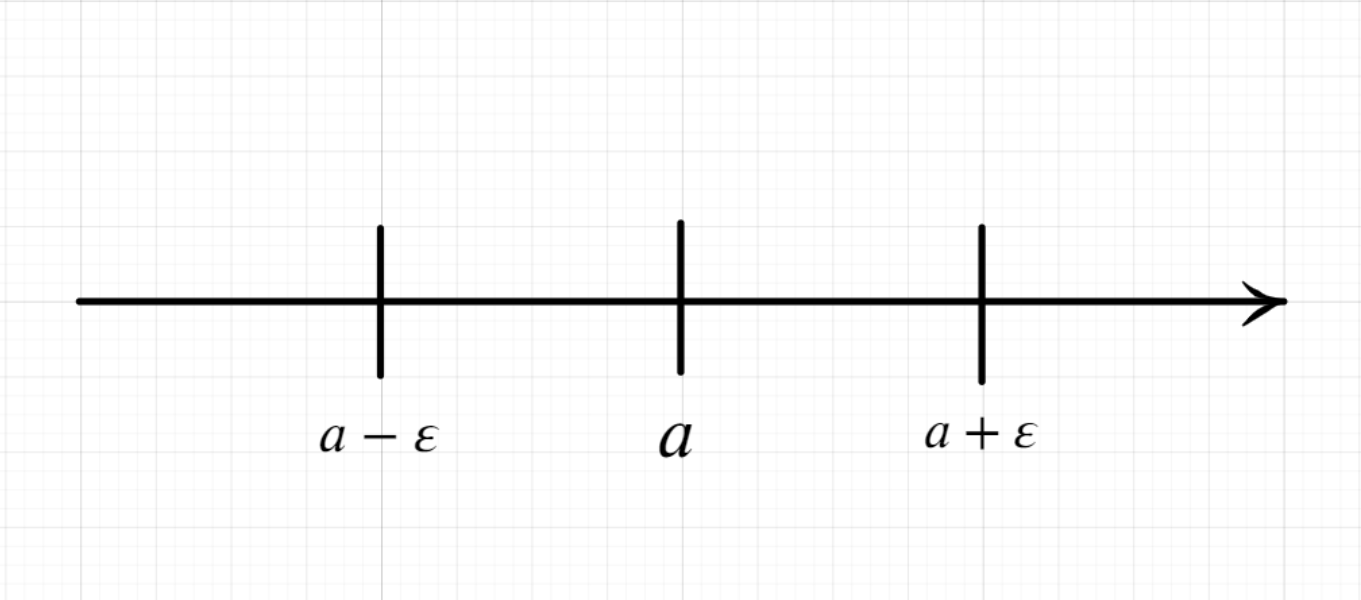
\includegraphics[scale=0.4]{images/img6.png}$$
$$|a_n-a|\leqslant\varepsilon\Longleftrightarrow -\varepsilon\leqslant a_n-a \leqslant \varepsilon\Longleftrightarrow a-\varepsilon\leqslant a_n \leqslant a+\varepsilon.$$
То есть получили $\varepsilon$-окрестность точки $a$.\\\\
$\bullet$ \textit{Если $a_n \to a $ и $a_n>a$, $\forall n \geqslant \nu_\varepsilon$, то говорят, что $a_n$ \textbf{стремится} к $a$ \textbf{справа} и пишут $a_n\to a+0.$}\\\\
$\bullet$ \textit{Если $a_n \to a $ и $a_n<a$, $\forall n \geqslant \nu_\varepsilon$, то говорят, что $a_n$ \textbf{стремится} к $a$ \textbf{слева} и пишут $a_n\to a-0$.}\\\\
Эти определения можно сформулировать и на языке $"\varepsilon-\nu"$:\begin{center}
	$a_n\to a+0$, если $\forall\varepsilon>0$, $\exists\nu_\varepsilon>0$, $\forall n \geqslant\nu_\varepsilon\Rightarrow 0<a_n - a \leqslant \varepsilon$\\
	$a_n\to a-0$, если $\forall\varepsilon>0$, $\exists\nu_\varepsilon>0$, $\forall n \geqslant\nu_\varepsilon\Rightarrow 0<a - a_n \leqslant \varepsilon$.
\end{center}
\section{Свойства сходящихся последовательностей.}
\begin{enumerate}
	\item \textbf{Необходимое условие сходимости последовательности.}\\
	\textit{Если $(a_n)$ сходится, то она ограничена.}
	\begin{Proof}
		$a_n=a+\alpha_n \Rightarrow |a_n|=|a+\alpha_n|\leqslant|a|+|\alpha_n|$.
	\end{Proof}
	\item \textbf{Единственность предела.}\\
	\textit{Сходящаяся последовательность имеет только один предел.}
	\begin{Proof}
		Пусть $a_n\to a$ и $a_n \to b$ тогдa\\
		$a_n=a+\alpha_n$ и $a_n=b+\beta_n\Rightarrow 0=a-b\ +$ бмп $\Rightarrow a-b=$ бмп $\Rightarrow a-b=0 \Rightarrow a=b$.
	\end{Proof}
	\item \textit{Изменение конечного числа членов последовательности не нарушает сходимости и не меняет величинины предела, если он существует.}
	\begin{Proof}
		Пусть ($a_n$), $\lim a_n = a$.
		Тогда $$\forall \varepsilon > 0,\ \exists\nu_\varepsilon,\ \forall n \geqslant \nu_\varepsilon \Rightarrow |a_n-a| \leqslant\varepsilon.$$
		Изменим конечное число членов последовательности. Тогда $\exists\mu$, что для $\forall n \geqslant \mu$ члены последовательности не измeнились. A тогда $$\forall n \geqslant\nu_1 ::=\max\{\nu_\varepsilon,\mu\}\ \Rightarrow|a_n-a|\leqslant\varepsilon.$$
	\end{Proof}
	\item \textit{Если $a_n \to a, b_n \to b$ и $A$ и $B$ -- постоянные,то $A\cdot a_n + B\cdot b_n \to A\cdot a + B \cdot b$ (предел линейной комбинации равен линейной комбинации пределов).}
	\begin{Proof}
		Пусть $a_n=a+\alpha_n,\ b_n=b+\beta_n$.\\
		Тогда $A\cdot a_n + B \cdot b_n = A(a+\alpha_n)+B(b+\beta_u)=Aa+Bb+\underbrace{A\alpha_n+B\beta_u}_{\text{бмп}}.$
	\end{Proof}
	\item \textit{$(a_n \to a, b_n \to b)$ $\Rightarrow a_n b_n \to ab$.}
	\begin{Proof}
		$a_n b_n=(a+\alpha_n)(b+\beta_n)=ab+\underbrace{a\beta_u+b\alpha_n+\alpha_n\beta_n}_{\text{бмп}}$.
	\end{Proof}
	\item \textit{Если $a_n \to a,\ b_n \to b$ и $b_n \neq 0,\ \forall n ,\ b \neq 0$, то $\dfrac {a_n}{b_n} \to \dfrac {a} {b} $, то есть предел частного равен частному пределов, если эти пределы существуют.}
	\begin{Proof}
		Сначала докажем, что $\dfrac {1}{b_n} \to \dfrac {1}{b}.$ Докажем, что $\Big(\dfrac {1}{b_n}\Big)$ ограничена. Действительно, так как $b_n \to b$, то $$\forall \varepsilon > 0,\ \exists \nu_\varepsilon,\ \forall n \geqslant \nu_\varepsilon \Rightarrow |b_n - b| \leqslant \varepsilon.$$
		Предположим здесь $\varepsilon:=\dfrac{|b|}{2}.$ Тогда, начиная с некоторого номера $|b_n-b|\leqslant\dfrac{|b|}{2}$, или, записывая двойным неравенством, имеем $$b-\dfrac{|b|}{2}\leqslant b_n\leqslant b+\dfrac{|b|}{2}.$$
		Для $b> 0$ $$\dfrac{b}{2}\leqslant b_n \leqslant \dfrac{3b}{2}\Rightarrow b_n \geqslant \dfrac{|b|}{2}.$$
		Для $b< 0$ $$\dfrac{3b}{2}\leqslant b_n \leqslant \dfrac{b}{2}\Rightarrow b_n \geqslant -\dfrac{|b|}{2}.$$
		Или
		$$\begin{cases}
			b_n \geqslant \dfrac {|b|}{2},\\
			b_n \leqslant -\dfrac {|b|}{2}
		\end{cases}  \Longleftrightarrow |b_n| \geqslant \dfrac {|b|}{2}.$$
		Поэтому $\dfrac {1}{|b_n|} \leqslant \dfrac {2}{|b|}$.\\
		Доказали, что один из остатков последовательности $\Big(\dfrac {1}{b_n}\Big)$ ограничен $\Rightarrow$ ограничена и вся последовательность.
		Теперь рассмотрим $\dfrac {1}{b_n} - \dfrac {1}{b}=\underset{\text{бмп}}{(b-b_n)}\cdot\dfrac {1}{\underset{\text{огр.}}{b\cdot b_n}} \Rightarrow$ бмп.\\
		Таким образом $\dfrac {1}{b_n} = \dfrac {1}{b}$ + бмп $\Rightarrow$ $\dfrac {1}{b_n} \to \dfrac {1}{b}$.\\
		Тогда $\dfrac {a_n}{b_n}=a_n\dots\dfrac {1}{b_n}\to \dfrac {a}{b}$ по свойству 5.
	\end{Proof}
\end{enumerate}
\section{Переход к пределу в неравенствах.}
\begin{lem}[Лемма о сжатой переменной]
	\begin{enumerate}
		\item Если $a_n\leqslant b_n \leqslant c_n$, для $\forall n $ и $a_n \to a, c_n \to a \Rightarrow (b_n)$ сходится и $\lim b_n = a$.
		\item  Пусть последовательности $(x_n)$ и $(y_n)$ сходятся, причём $x_n \to a, y_n \to b$. Если $a<b$, то найдется $\nu$, что $\forall n \geqslant \nu_\varepsilon \Rightarrow x_n < y_n$.
		\item Пусть $x_n \to a, y_n \to b$.\\
		Если $\exists\nu$ такие, что при $\forall n \geqslant\nu$ выполняется\begin{enumerate}
			\item $x_n>y_n\Rightarrow a \geqslant b$;
			\item $x_n \geqslant y_n\Rightarrow a \geqslant b$;
			\item $x_n>b\Rightarrow a \geqslant b$;
			\item $x_n\geqslant b \Rightarrow a \geqslant b$.
		\end{enumerate}
	\end{enumerate}
\end{lem}

\begin{Proof}
	\begin{enumerate}
		\item
		$\begin{matrix}
			a_n \to a\\
			c_n \to a 
		\end{matrix} \Rightarrow \forall \varepsilon > 0,\ \begin{matrix}
			\exists \nu_\varepsilon^{(1)},\ \forall n \geqslant\nu_\varepsilon^{(1)}\Rightarrow a-\varepsilon \leqslant a_n;\\
			\exists \nu_\varepsilon^{(2)},\ \forall n \geqslant\nu_\varepsilon^{(2)}\Rightarrow  c_n \leqslant a+\varepsilon.
		\end{matrix}$\\\\
		Тогда $a-\varepsilon\leqslant a_n\leqslant b_n \leqslant c_n \leqslant a+\varepsilon$, то есть
		$$\forall\varepsilon>0,\ \exists\nu (\varepsilon ) ::= \max \{\nu_\varepsilon^{(1)},\nu_\varepsilon^{(2)}\}, \forall n \geqslant \nu_\varepsilon \Rightarrow |b_n - a| \leqslant \varepsilon.$$
		\item Возьмём $\varepsilon:=\dfrac{b-a}{3}.$ По определению предела $\exists \nu_1, \forall n \geqslant\nu_1 \Rightarrow |x_n-a| \leqslant \dfrac{b-a}{3}$ и $\exists\nu_2,\forall n \geqslant\nu_2 \Rightarrow$
		$|y_n-b|\leqslant\dfrac{b-a}{3}$. Toгда
		$$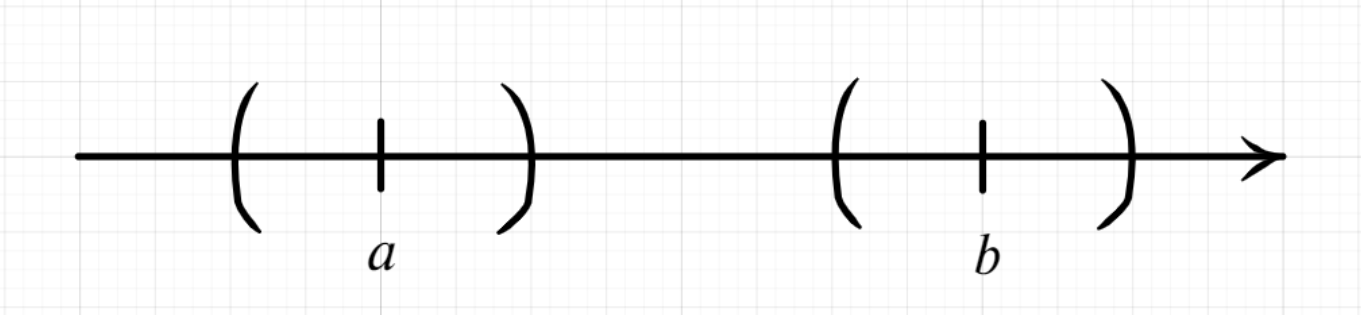
\includegraphics[scale=0.4]{images/img7.png}$$
		$$x_n\leqslant a+\frac{b-a}{3}<b-\frac{b-a}{3}\leqslant y_n,$$ то есть
		$x_n<y_n$ для $n\geqslant\max\{\nu_1,\nu_2\}$.
		\item Рассуждая от противоположного из 2 сразу же вытекает а) и b); c) и d) --- частные случаи a) и b), полученные при $y_n=b$.
	\end{enumerate}
\end{Proof}\\
\begin{example}
	$\dfrac{1}{n}>0$ при $\forall n \in \N,$ однако $\lim\dfrac{1}{n}=0$.\\
	Знак строго неравенства при переходе к пределу не сохраняется.\end{example}   
\section{Монотонные последовательности.}
$\bullet$ \textit{Последовательность $(a_n)$ будем называть}
\begin{enumerate}
	\item \textit{\textbf{возростающей},если для} $n_2>n_1\Rightarrow a_{n2}\geqslant a_{n1}(a_n\leqslant a_{n+1})$;
	\item \textit{\textbf{строго возрастающей}} $n_2>n_1\Rightarrow a_{n2} > a_{n1}(a_n < a_{n+1})$;
	\item \textit{\textbf{убывающей}} $n_2>n_1\Rightarrow a_{n2} \leqslant a_{n1}(a_n\geqslant a_{n+1})$;
	\item \textit{\textbf{строго убывающей}}, $n_2>n_1\Rightarrow  a_{n2} < a_{n1}(a_n > a_{n+1})$
\end{enumerate}
\textit{1, 3 --- \textbf{монотонные} 2, 4 --- \textbf{строго монотонные}}.\\\\
Иногда применяют другую терминологию:\\
1 --- неубывающие; 2 --- возврастающие; 3 --- невозврастающие; 4 --- убывающие.
\begin{theorem} [Теорема о пределе монотонной последовательности.]
	Любая ограниченная монотонная последовательность имеет конечный предел.
\end{theorem}
\begin{Proof}
	Доказательство преведем для возрастающей последовательности.\\\\
	Пусть ($a_n$) возрастает и ограничена сверху. Так как ($a_n$) ограничена, то $\exists M$, что $a_n\leqslant M$, $\forall n$. Так как ($a_n$) возрастает, то $a_{n+1}\geqslant a_n$.\\\\
	Рассмотрим множество $\{a_n\}$. Это множество не пусто и ограничено сверху. Следовательно, по теореме о границах $\exists \sup \{a_n\}$.
	Обозначим $a::=\sup\{a_n\}$. Так как $a$ --- верхняя граница, то \begin{enumerate}
		\item $\forall n \Rightarrow a_n \leqslant a$;
		\item $\forall\varepsilon > 0,\exists \bar n, a_{ \bar n}> a - \varepsilon$.
	\end{enumerate}
	Рассмотрим $a_n$ для $n\geqslant \bar n$\begin{center}
		$a_n\geqslant a_{ \bar n}>a-\varepsilon$ и $a_n\leqslant a\leqslant a+\varepsilon$.
	\end{center}
	Таким образом, $a-\varepsilon\leqslant a_n\leqslant a+\varepsilon$ и окончательно.
	$$\forall\varepsilon >0,\exists\bar n ,\forall n \geqslant \bar n \Rightarrow |a_n - a|\leqslant\varepsilon.$$
\end{Proof}\\
Следовательно, $a=\lim a_n$. Аналогично доказывается теорема и для случая ограниченной снизу последовательности.
\begin{theorem}
	Если последовательность $(a_n)$ монотонно возрастает и неограничена сверху, то она является бесконечно большой.
\end{theorem}
\begin{Proof}
	Действительно, так как она неограничена, то $\forall\varepsilon > 0,\exists\bar n ,$ что $a_{\bar n}\geqslant\varepsilon$. Но $a_n \geqslant a_{\bar n}\geqslant\varepsilon$\\
	и для $\forall n \geqslant \bar n \Rightarrow (a_n)$ --- ббп.
\end{Proof}\\\\
Для ббп, мы уже говорили, пишут $\lim a_n = \infty$. Если же $(a_n)$ --- ббп и $a_n>0,\forall n \geqslant \nu_\varepsilon$,\\
то $\lim a_n = +\infty$, если $(a_n)$ --- ббп и $a_n < 0,\forall n \geqslant \nu_\varepsilon$, то $\lim a_n = -\infty$.\\\\
Итак, если $a_n$ возрастает и неограничена сверху, то $\lim a_n = +\infty$.\\
Аналогично: если $a_n$ убывает и неограничена снизу, то $\lim b_n = -\infty$.\\\\
\textbf{Вывод.} Монотонная последовательность всегда имеет предел. Если последовательность ограничена, то предел конечный, т.е. последовательность сходится.
\begin{center}
	\textbf{Возможности}
\end{center}
Последовательность имеет предел, если существует конечный или бесконечный предел. Последовательность сходится, если предел конечный. Если предел последовательности не существует, то она не имеет предела. В случае, если последовательность имеет бесконечный предел или предела не сущесвует, последовательность расходится
\section{Число e.}
Рассмотрим последовательность $a_{n}$, где
$$a_{n} = (1 + \dfrac{1}{n})^n.$$
\begin{enumerate}
	\item $(a_{n})$ \textit{монотонна}.\\\\ Чтобы доказать это, распишем $a_{n}$ по формуле Ньютона\\
	\\$a_{n} = (1 + \dfrac{1}{n})^n  = 1 + 1 + \dfrac{n\cdot(n -1)}{2!}\cdot\dfrac{1}{n^2} + \ldots + \dfrac{n\cdot(n - 1)\dots(n- \beta + 1)}{\beta!}\cdot\dfrac{1}{n^\beta} + \ldots + \dfrac{n\dot(n-2)\dots 1}{n!}\cdot\dfrac{1}{n^n} = 1 + 1 + \dfrac{1}{2!} \cdot(1 - \dfrac{1}{n}) + \ldots + \dfrac{1}{\beta!}\cdot(1-\dfrac{1}{n})\cdot(1-\dfrac{2}{n})\dots(1-\dfrac{\beta - 1}{n}) + \ldots + \dfrac{1}{n!}\cdot(1-\dfrac{1}{n})\cdot(1-\dfrac{2}{n}) \dots (1-\dfrac{n - 1}{n})$\\
	\\
	Аналогично\\
	\\$a_{n+1} =(1 + \dfrac{1}{n + 1})^n = 1 + 1 + \dfrac{1}{2!} \cdot(1 - \dfrac{1}{n + 1}) + \ldots + \dfrac{1}{\beta!}\cdot(1-\dfrac{1}{n + 1})\cdot(1-\dfrac{2}{n + 1})\dots(1-\dfrac{\beta - 1}{n + 1}) + \ldots + \dfrac{1}{(n + 1)!}\cdot(1-\dfrac{1}{n + 1}) \dots (1-\dfrac{n}{n +1}) $\\
	\\
	Сравним $a_{n}$ и $a_{n + 1}$.\\\\
	Каждое слагаемое в $a_{n + 1}$ больше соответсвующего слагаемого в $a_{n}$, кроме того, в $a_{n + 1}$ на одно слагаемое больше. Отсюда следует, что $a_{n + 1} $ > $a_{n}$, то есть ($a_{n}$) строго возрастает.
	\item $(a_{n})$ \textbf{ограничена}.\\\\
	\\$a_{n} < 2 + \dfrac{1}{2!} + \dfrac{1}{3!} + \dots + \dfrac{1}{\beta!} + \dots + \dfrac{1}{n!} < 2 + \dfrac{1}{2} + \dfrac{1}{2^2}+ \ldots + \dfrac{1}{2^{(n - 1)}} < 2 + \dfrac{1}{2} + \dfrac{1}{2^2} + \ldots = 1 + \dfrac{1}{1- \frac{1}{2}} = 3$.\\
	Итак 2 < $a_{n }$ < 3.\\
\end{enumerate}
Значит, на основании теоремы предыдущего пункта у последовательностей ($a_{n}$) cуществует конечный предел. Следуя Эйлеру, его обозначают символом $e$, то есть
\begin{center}
	$e ::= \lim\limits_{n\to\infty} \Big(1 + \dfrac{1}{n}\Big)^n$
\end{center}
Оно равно $e = 2.718281828409045\dots$, функция $e^x$ --- экспонента. Логарифм по основанию $е$ --- натуральный логарифм: $\ln x ::= \log_e x $\\
$M::=\lg e = \dfrac{1}{\ln10} = 0.4342944819\dots$\\
$\log_{10} x = \dfrac{\ln x}{\ln10} = M\cdot \ln x$;\quad
$\ln x = \dfrac{\lg x}{\lg e}$\\
\\\textit{
	$\bullet$ В связи с натуральным основанием $е$ рассматривают функции, которые называют \textbf{гиперболическими функциями}:}\\
$$ \sh x = \dfrac{e^x - e^{-x}}{2};\quad \ch x = \dfrac{e^x + e^{-x}}{2}$$
$$\th x = \dfrac{\sh x}{\ch x};\quad \cth x = \dfrac{\ch x}{\sh x}$$
Названия у функций сходные с тригонометрическими и обозначения похожи, потому что эти функции обладают рядом аналогичных свойств\\
Например: $\ch^2 x - \sh^2 x = \Big(\dfrac{e^x + e{-x} }{2}\Big)^2 - \Big(\dfrac{e^x - e^{-x} }{2}\Big)^2 = \dfrac{e^x + 2 + e^{-2x}}{4} - \dfrac{e^{2x} - 2 + e^{-2x}}{4} = 1$.
\begin{center}
	$\ch^2 x - \sh^2 x = 1$.
\end{center}
Аналогично доказываются и такие формулы:
$$ \sh^2x + \ch^2x = \ch2x,\quad2\cdot \sh x \cdot \ch x = \sh2x$$ и так далее\\\\
Например, $\sh(x + y)$, $\ch(x + y)$ рассчитываются по формулам, аналогичным формулам тригонометрии.\\
Подробнее в $"$Основные математические формулы$"$.
\section{Подпоследовательности.}
$\bullet$ \textit{Последовательность $(b_k)$ называется \textbf{подпоследовательностью} последовательности $(a_n)$, если для $\forall \Rm \in\mathbb{N}$ $\exists n_k  
	\in\mathbb{N}$, что $b_k = a_{nk}$, и при этом $n_1 < n_2 <\dots$.}\\\\
Для обозначения подпоследовательности чаще всего используется символ ($a{nk}$) = ($a_{n1}, a_{n2}, \dots$)
Должен сохранятся существующий порядок. Любой остаток последовательности является подпоследовательностью.\\
\begin{example}
	$(a_n) = (1, 2, 3, 4, \dots , n , \dots) $\\
	$(1, 3 ,5 ,7, \dots , 2\cdot n - 1, \dots )$ --- подпоследовательность.\\
	$(3, 1 , 5 , 7 , \dots, 2\cdot k - 1, \dots )$ --- не является подпоследовательностью.
\end{example}
\begin{theorem}
	Если последовательность $(a_n)$ сходится к числу а, то любая её подпоследовательность тоже сходится, причём к тому же пределу.
\end{theorem}
\begin{Proof}
	Рассмотрим последовательность $(a_n)$. Введём подпоследовательность $(a_{nk})$. Так как  $\lim a_n = a$, то $$\forall\varepsilon > 0,\ \exists \nu_\varepsilon, \forall n \geqslant \nu_\varepsilon \Rightarrow | a_n - a| \leqslant \varepsilon.$$
	Рассмотрим $k\geqslant \nu_\varepsilon \Rightarrow n_k \geqslant \nu_\varepsilon \Rightarrow |a_{nk} - a| \leqslant\varepsilon.$
	Итак, $$\forall \varepsilon > 0,\ \exists k,\ \forall k \geqslant \nu \varepsilon \Rightarrow |a_{nk} - a| \leqslant \varepsilon \Rightarrow \lim\limits_{k\to\infty} a_{nk} = a.$$
\end{Proof}
\begin{theorem}
	[о монотонной подпоследовательности]
	Из любой последовательности можно извлечь монотонную подпоследовательность.
\end{theorem}
\begin{Proof}\begin{enumerate}
		\item Пусть ($a_n$) обладает остатком ($a_m , a_{m + 1} , \dots, a_{m + l} \dots $), причём этот остаток не имеет наибольшего элемента. Тогда и любой послдующий остаток не имеет наибольшего элемента
		$$a_{n1} ::= a_m$$
		и выберем $n_2$ так, чтобы $a_{n2} > a_{n1}$.
		Из остатка ($a_{n2} , a_{n2 + 1}$) выберем $a_{n3} > a_{n2}$ и т.д. Построенная таким образом подпоследовательность является возрастающей (строго возрастащей).
		\item Пусть любой остаток обладает наибольшим элементом. Обозначим $a_{n_1}$ наибольший элемент последовательности ($a_n$). Рассмотрим остаток ($a_{n1 + 1} , a_{n1 + 2}$).
		Пусть $a_{n2}$ --- наибольший элемент этого остатка:
		$$a_{n1} \geqslant a_{n2}$$
		Далее рассматриваем остаток ($a_{n2 + 1}, \dots$) и повторяем описанную процедуру.
	\end{enumerate}
	($a_{nk}$) --- убывающая последовательность.
\end{Proof}
\section{Принцип выбора.}
\begin{thbv} [принцип выбора]
	Из любой ограниченной последовательности можно извлечь сходящуюся последовательность.
\end{thbv}
\begin{Proof}
	Из ($a_n$) на основании теоремы о монотонной последовательности можно извлечь монотонную подпоследовательность ($a_{nk}$). Поскольку ($a_n$) ограничена, то ограничена и ($a_{nk}$). А т.к. ($a_{nk}$) монотонна и ограничена, то у неё существует конечный предел.
\end{Proof}
\\\\
Теорема утверждает, что любая ограниченная последовательность обладает хотя бы одним пределом.\\\\ 
Таким образом, из любой последовательности можно выделить подпоследовательность, имеющую предел. При этом, если последовательность ограничена, то предел конечен, а если неограничен, то предел бесконечен.
\section{Критерий Коши сходимости последовательности.}
Довольно часто относительно данной последовательности нам приходится выяснять, является ли она сходящейся. Не находить предел, а только ответить на вопрос, сходится она или нет. По определению такую задачу решать неудобно, поскольку в него входит значение предела, которое наперёд может быть и неизвестно, а найти его не всегда просто. Неплохо бы иметь возможность на основании только свойств элементов последовательности, определить сходится она или нет. К изучению этого вопроса мы сейчас и переходим.\\\\
$\bullet$ Г\textit{оворят, что последовательность $(a_n)$ \textbf{удовлетворяет условию Коши}, если}
$$\forall \epsilon > 0,\ \exists \nu_\epsilon ,\ \forall n,\ m \ge \nu_\epsilon \Rightarrow |a_n - a_m| \le \epsilon.\eqno(*)$$
\textit{Условие $(*)$ можно заменить и равносильным}
$$\forall \epsilon > 0,\ \exists \nu_\epsilon ,\ \forall n \ge \nu_\epsilon,\ \forall p \ge 0 \Rightarrow |a_{n+p} - a_n| \le \epsilon.$$
Для доказательства равносильности этих двух условий достаточно положить $p=n-m$ или $p = m-n$.\\\\
В условии Коши участвуют только члены последовательности ($a_n$), это условие отображает внутреннее свойство последовательности.\\\\
$\bullet$ \textit{Последовательность, удолетворяющую условию Коши, называют также \textbf{фундаментальной последовательностью.}}
\begin{lemma}[M-лемма для условия Коши]
	Если $$\forall \epsilon > 0,\ \exists \nu_\epsilon,\ \forall n,\ m \ge \nu_\epsilon \Rightarrow |a_n - a_m| \le M\cdot \epsilon,$$ где $M$ не зависит ни от $n$, ни от $m$, ни от $\epsilon$, то $(a_n)$ фундаметальна. 
\end{lemma}
\begin{theorem}[Критерий Коши]
	Для сходимости  последовательности $(a_n)$ необходимо и достаточно чтобы она была фундаметнальной.   
\end{theorem}
\begin{Proof}
	\textbf{Необходимость.} Дано: ($a_n$) сходится $\Rightarrow \exists a \in \Rm$ такое, что $$\forall \epsilon > 0, \exists \nu_\epsilon, \forall n \ge \nu_\epsilon \Rightarrow |a_n - a| \le \epsilon$$ и $$\forall m \ge \nu_\epsilon \Rightarrow |a_m - a| \le \epsilon.$$
	Тогда $$|a_n - a_m| = |(a_n - a)-(a_m - a)| \le |a_n - a| + |a_m - a| \le 2\cdot\epsilon,\quad \forall n, m \ge \nu_\epsilon.$$ Итак, $$\forall \epsilon > 0, \exists \nu_\epsilon, \forall n,m \ge \nu_\epsilon \Rightarrow |a_n - a_m| \le 2\cdot\epsilon.$$
	На основании  М-леммы для условия Коши это и означает, что ($a_n$) фунаментальна.\\\\
	\textbf{Достаточность.} Пусть $(a_n)$ фундаметнальна. А это значит, что ($a_n$) cходится.\\
	Докажем сначала, что ($a_n$) ограничена. Из фундаметнальности ($a_n$) вытекает, что $$\forall\epsilon > 0, \exists \nu_\epsilon, \forall n, m \ge \nu_\epsilon \Rightarrow |a_n - a_m| \le \epsilon$$
	Положим $\epsilon := 1$, $|a_n - a_m|\le1$, отсюда $a_m - 1 \le a_n \le a_m + 1$.
	Зафиксируем $m \ge \nu_\epsilon$. Тогда один из остатков последовательности ($a_n$) ограничен $\Rightarrow$ ограничена и вся ($a_n$).\\
	На основании принципа выбора из ($a_n$) можно выделить сходящуюся последовательность.\\
	($a_{nk}$), $a::= \lim\limits_{k\to\infty} a_{nk}$.
	В силу фундаментальности ($a_n$): $$\forall\epsilon > 0, \exists\nu_\epsilon, \forall n,n_k \ge \nu_\epsilon \Rightarrow |a_n - a_{nk}| \le\epsilon$$ или $$
	a_{nk} - \epsilon \le a_n \le a_{nk} + \epsilon.$$
	Перейдём в этом неравенстве к пределу при $k \to \infty$. Тогда и в $n_k \to \infty$ и получаем $$a - \epsilon \le a_n \le a + \epsilon.$$
	Таким образом $$\forall\epsilon > 0, \exists\nu_\epsilon, \forall n \le \nu_\epsilon \Rightarrow |a_n - a| \le \epsilon.$$ Это и означает, что ($a_n$) сходится.    
\end{Proof}\\
\begin{example}
	\begin{enumerate}
		\item Построим отрицание к условию Коши.\\
		условие Коши: $\forall \epsilon > 0, \exists \nu(\epsilon) , \forall n,m \ge \nu(\epsilon) \Rightarrow |a_n - a_m| \le \epsilon$;\\
		отрицание: $\exists \epsilon_0 > 0, \forall \nu({\epsilon_0}),\ \exists n^*,m^* \ge \nu({\epsilon_0}) \Rightarrow |a_{n^*} - a_{m^*}| > \epsilon_0$.\\
		\item Иследовать сходимость последовательности ($a_n$), где $a_n = 1 + \dfrac{1}{2} + \dfrac{1}{3} + \dots + \dfrac{1}{n}$.\\
		Рассмотрим $|a_{2n} - a_n| = \dfrac{1}{n + 1} + \dfrac{1}{n + 2} + \cdot + \dfrac{1}{n + n} > \dfrac{n}{n + n} = \dfrac{1}{2}$.\\
		Таким образом 
		$\exists \epsilon_0 = \dfrac{1}{4},\ n,\ \exists m = 2\cdot n \Rightarrow |a_m - a_n| > \dfrac{1}{4}.$\\
		Это и означает, что ($a_n$) расходится.
	\end{enumerate}
\end{example}  
\section{Верхний предел последовательности.}
Рассмотрим последовательность ($a_n$). Обозначим $\Rm_\infty = \Rm\cup\{-\infty ; \infty\}= [-\infty ; +\infty]$.\\\\
$\bullet$ \textit{Число $\alpha \in R_\infty$ будем называть \textbf{частным (частичным) пределом последовательности $(a_n)$}, если из $(a_n)$ можно извлечь подпоследовательность, имеющую пределом $\alpha$ $$ (a_n),\ (a_{nk}),\ a_{nk} \to \alpha,\ k \to \infty.$$ $\alpha$ может быть как конечным числом, так и символом $+\infty$ или $-\infty$.}\\\\
Обозначим $E$ --- множество частичных пределов последовательности ($a_n$), множество $E$ не пусто. Это следует из принципа выбора.\\\\
$\bullet$ \textit{Наибольший частный предел последовательности $(a_n)$ называется её \textbf{верхним пределом} и обозначается $\overline{\lim}\ a_n$, а наименьший частный предел называтеся \textbf{нижним пределом} и обозначатся $\underline{\lim}\ a_n$.}\\\\
Верхний и нижние пределы всегда существуют.
\begin{center}
	$\overline{\lim}\ a_n = \sup E$,\quad $\underline{\lim}\ a_n = \inf E$
\end{center}
Если последовательность ($a_n$) ограничена, то $\overline{\lim}\ a_n$ конечен, если же неограничена сверху, то $\overline{\lim}\ a_n = +\infty$. Поскольку $E$ не пусто, то $\underline{\lim}\ a_n \le \overline{\lim}\ a_n$ (так как $\sup \ge \inf$).
\begin{theorem}
	Для того, чтобы последовательность $(a_n)$ имела предел, необходимо и достаточно выполнение равенства $\overline{\lim}\ a_n = \underline{\lim}\ a_n$.\\
\end{theorem}
\begin{Proof}
	\textbf{Необходимость.} Пусть ($a_n$) имеет предел. Тогда любая её подпоследовательность имеет такой же предел $\Rightarrow E$ состоит из одного элемента, поэтому $\overline{\lim}\ a_n = \underline{\lim}\ a_n$.\\\\
	\textbf{Достаточность.} Пусть $\overline{\lim}\ a_n = \underline{\lim}\ a_n = ::a \Rightarrow E$ состоит из одного элемента, что означает, что всякая подпоследовательность из ($a_n$) сходится к одному и тому же пределу $\Rightarrow (a_n)$ сходится к тому же пределу (возьмём в качестве подпоследовательности остаток последовательности ($a_n$)).
\end{Proof}
\begin{theorem}
	Для того, чтобы число а было верхним пределом последовательности $(a_n)$, необходимо и достаточно выполнение двух условий
	\begin{enumerate}
		\item $\forall \epsilon > 0, \exists \nu_\epsilon, \forall n \ge \nu_\epsilon \Rightarrow a_n \le a + \epsilon$;
		\item $\forall \epsilon > 0, \forall n_0, \exists n'(\epsilon, n_0), n'> n_0 и a_{n'} > a - \epsilon$.
	\end{enumerate}
	Условие $1$ означает, что $\forall \epsilon > 0$ в последовательности $(a_n)$ существует лишь конечное число элементов, которые больше чем $a + \epsilon$ (их номера < $\nu_\epsilon$).\\\\
	Условие 2 означает, что $\exists$ бесконечно много членов последовательности $(a_n)$ таких, что $a_n > a - \epsilon$.\\
\end{theorem}
\begin{Proof} \textbf{Необходимость.}
	\begin{enumerate}
		\item  $a = \overline{\lim}\ a_n \Rightarrow \exists(a_{nk})$ такая, что $\lim\limits_{k\to\infty} a_{nk} = a$ и всякая другая сходящаяся подпоследовательность последовательности ($a_n$) имеет не больший предел
		$$\forall\epsilon > 0, \exists\nu_\epsilon, \forall k \ge \nu_\epsilon \Rightarrow a - \epsilon \le a_{nk} \le a + \epsilon.$$
		Предположим от противного, что бесконечное число членов последовательности ($a_n$)  удолетворяет условию $a_n \ge a + \epsilon$. Построим последовательность ($b_k$) из этих членов, являющуюся подпоследовательностью последовательности ($a_n$). Из последовательности ($b_k$) можно выделить подпоследовательность, имеющую предел, причём эта подпоследовательность является и подпоследовательность последовательности ($a_n$). Предел этой последовательности $\ge a + \epsilon$, что противоречит тому, что $a = \overline{\lim}\ a_n$\\
		\item вытекает из неравенства $a - \epsilon \le a_{nk}$.
	\end{enumerate}
	\textbf{Достаточность.}\begin{enumerate}
		\item $\forall n \ge \nu_\epsilon \quad  a_n \le a + \epsilon$;
		\item $\forall \epsilon > 0, \forall n_0, \exists n' = n'(\epsilon, n_0), n'\ge a_{n'} > a - \epsilon$.\\
		Построим подпоследовательность последовательности ($a_n$) по правилу: $n_0 = 1,\   \exists n_1,\   a_{n1} > a - \epsilon$.\\\\
		Рассмотрим остаток ($a_n) \dots (a_{n1}, \dots)$ и возьмём $n_0 = n + 1,\ \exists a_n > a - \epsilon.$\\\\
		Для ($a_{nk}$) $a - \epsilon < a_{nk} < a + \epsilon \Rightarrow \lim a_{nk} = a$. $a$ --- наибольший частичный предел. От противного, если $\exists b > a$, то возникает противоречие пункту 1.
	\end{enumerate}
\end{Proof}
\section{Числовые ряды.}
Возьмём последовательность ($a_n$) и исходя из неё построим последовательность ($s_n$) по следующему правилу:
\begin{center}
	$s_1 = a_1;\quad s_2 = a_1 + a_2;\quad s_3 = a_1 + a_2 + a_3;\quad \ldots \quad s_n = a_1 + a_2 + \dots +a_n;$.
\end{center}
$\bullet$\textit{ Последовательность $(s_n)$ записывают в виде единого символа
	\begin{center}
		$a_1 + a_2 + \ldots + a_n + \ldots = \sum\limits_{n=1}^\infty a_n$
	\end{center}
	и называют \textbf{рядом}.}\\\\
Обозначают $a_n$ --- $n$-ый член ряда, $s_n$ --- частичная сумма ряда.\\\\
$\bullet$ \textit{Если последовательность $(s_n)$ сходится, то ряд называют \textbf{сходящимся}, а $\lim\limits_{n\to\infty} s_n$ называют \textbf{суммой ряда}. В этом случае пишут:}
\begin{center}
	$\sum\limits_{k=1}^\infty a_k = s.$
\end{center}
$\bullet$ \textit{Если же $\lim s_n$ не существует либо бесконечен, то ряд называют \textbf{расходящимся.}}\\\\
% 50 - 60
Если $\lim s_n = \infty$, то иногда пишут $\sum\limits_{k=1}^{\infty}a_k=\infty$.\\
\begin{example}
	\\$\sum\limits_{n=0}^\infty q^k = 1 + q + q^2 + \ldots + q^n + \ldots$\\
	$S_n = 1 + q + \ldots + q^{n-1} = \dfrac{1-q^n}{1-q}\quad\Ra\quad \lim\limits_{n\to\infty}S_n=\dfrac{1}{1-q}$, если $|q|<1.$\\
	Если же $|q|>1$, то ряд расходится.
\end{example}\\\\
Из критерия Коши сходимости последовательности вытекает
\begin{theorem}
	[критерий Коши сходимости ряда]
	Для сходимости ряда $\sum\limits_{n=1}^{\infty}a_n$ необходимо и достаточно, чтобы последовательность его частных сумм была фундаментальной, т.е.
	$$\forall\varepsilon>0, \exists\nu_\varepsilon, \forall n\geqslant\nu_\varepsilon, \forall p\geqslant0\Ra|S_{n+p}-S_n|\leqslant\varepsilon.$$
\end{theorem}
Но $|S_{n+p}-S_{n}| = |\sum\limits_{k=1}^{n+p}a_k-\sum\limits_{k=1}^{n}a_k|=|\sum\limits_{k=n+1}^{n+p}a_n|\leqslant\varepsilon.$\\\\
Таким образом,\\\\
\textit{Для сходимости ряда $\sum a_k$ необходимо и достаточно} \textit{чтобы} $$\forall\varepsilon>0,\ \exists\nu_\varepsilon,\ \forall n \geqslant\nu_\varepsilon,\ \forall p\geqslant0\ \Ra |\sum\limits_{k=n+1}^{n+p}a_k|\leqslant\varepsilon.$$
Из последнего неравенства в частности вытекает при $p=1$ $|a_{n+1}|\leqslant\varepsilon$. Это означает, что последовательность $(a_n)$ --- бмп. Таким образом,
\newtheorem*{nys}{Необходимое условие сходимости ряда}
\begin{nys}
	Если $\sum a_n$ --- сходится, то $\lim a_n = 0$.
\end{nys}
\begin{example}
	\\$\sum\dfrac{1}{n^2}$,  $\Big|\sum\limits_{k=n+1}^{n+p}a_k\Big|=\dfrac{1}{(n+1)^2} + \ldots + \dfrac{1}{(n+p)^2} = \dfrac{1}{n(n+1)} + \ldots + \dfrac{1}{(n+p-1)(n+1)} = \dfrac{1}{n}-\dfrac{1}{n+p}\leqslant\dfrac{1}{n}\leqslant\varepsilon$
\end{example}
\section{Предел последовательности комплексных чисел.}
($c_n$) --- последовтельность комплексных чисел.\\
$$f:\mathbb{N}\rightarrow\mathbb{C},\ f(n) = ::c_n = a_n + ib_n$$
($c_n$) сходится, если: $\exists c \in \mathbb{C}$,
$$\forall\varepsilon,\exists\nu_\varepsilon,\forall n\geqslant\nu_\varepsilon\Ra|c_n-c|\leqslant\varepsilon$$
\newtheorem*{ks}{Критерий сходимости}
\begin{ks}
	Для того, чтобы $(c_n)$, $c_n=a_n+ib_n$ была сходящейся к числу $a+ib\lra a_n\rightarrow a$, $b_n\rightarrow b$.
\end{ks}
\begin{Proof}\\
	\textbf{Необходимость.} Пусть ($c_n$) сходится. Тогда $$\forall\varepsilon>0,\  \exists\nu_\varepsilon,\ \forall n\geqslant\nu_\varepsilon\Rightarrow|c_n-c|\leqslant\varepsilon.$$ Но $|c_n-c|=\sqrt{(a_n-a)^2+(b_n-b)^2}$. Тогда $|a_n-a| = \sqrt{(a_n-a)^2}\leqslant\sqrt{(a_n-a)^2+(b_n-b)^2}=|c_n-c|\leqslant\varepsilon\Ra a_n\rightarrow a$. Аналогично $b_n\rightarrow b$.\\\\
	\textbf{Достаточность.}
	$$a_n\rightarrow a\Rightarrow\forall\varepsilon>0,\ \exists\nu_1(\varepsilon), \forall n \geqslant \nu_1(\varepsilon)\Rightarrow|a_n-a|\leqslant\varepsilon;$$
	$$b_n\ra b\Ra\forall\varepsilon > 0,\ \exists\nu_2(\varepsilon),\ \forall n\geqslant\nu_2(\varepsilon)\Ra|b_n-b|\leqslant\varepsilon.$$\\
	Тогда для $n\geqslant\nu(\varepsilon)::=\max\{\nu_1,\nu_2\}$ будем иметь $|c_n - c|\leqslant\sqrt{(a_n-a)^2 + (b_n-b)^2}\leqslant\varepsilon\sqrt{2}.$
\end{Proof}\\\\
Для последовательностей комплексных чисел имеют место \textbf{принцип выбора}, \textbf{критерий Коши}, \textbf{арифмтеика приделов} и т.д.